% Journal layout from New_IEEEtran_how-to.tex; IEEEtran names letter size letterpaper.
\documentclass[letterpaper,journal]{IEEEtran}
\usepackage[T1]{fontenc}
\usepackage{amsmath,amssymb,array,booktabs,graphicx,url,listings,multirow,xcolor}
\usepackage{cite}
\usepackage{textcomp}
\usepackage{stfloats}
\usepackage{balance}
\usepackage{tikz}
\usetikzlibrary{positioning,fit,arrows.meta,calc,backgrounds}
\usepackage{algorithm}
\usepackage[noend]{algpseudocode}
\usepackage[hidelinks]{hyperref}
\lstset{basicstyle=\ttfamily\scriptsize,captionpos=b,abovecaptionskip=6pt,belowcaptionskip=2pt,breaklines=true,columns=fullflexible,frame=single,
  morekeywords={harness,component,evolution,operation,target,from,to,depends,parents,capabilities,requires,expect,ensure,version,mutable},
  keywordstyle=\bfseries,xleftmargin=2pt,xrightmargin=2pt,aboveskip=4pt,belowskip=2pt}
\algrenewcommand\algorithmicrequire{\textbf{Input:}}
\algrenewcommand\algorithmicensure{\textbf{Output:}}
\algnewcommand{\Req}{\textbf{require }}
\algrenewcommand\alglinenumber[1]{\scriptsize #1:}
\newcolumntype{L}[1]{>{\raggedright\arraybackslash}p{#1}}
\newcommand{\tool}{SSEVOH-DSL}
\newcommand{\harness}{Harness\textsuperscript{2}}
\pdfstringdefDisableCommands{\def\harness{Harness2}}
\newcommand{\pathcode}[1]{\nolinkurl{#1}}
\newcommand{\sv}[2]{\ensuremath{\langle\textsf{#1},#2\rangle}}
% numbered flow badges, pre-rendered so that captions never run TikZ
\makeatletter
\AtBeginDocument{\@for\n:={1,2,3,4,5,6,7,8,9}\do{%
  \expandafter\newsavebox\csname flowbadge\n\endcsname
  \global\expandafter\sbox\csname flowbadge\n\endcsname{\tikz[baseline=(c.base)]\node[circle,fill=black,text=white,inner sep=0.6pt,font=\scriptsize\bfseries](c){\n};}}}
\DeclareRobustCommand{\circled}[1]{\expandafter\usebox\csname flowbadge#1\endcsname}
\makeatother
\definecolor{trust}{HTML}{2A78D6}
\definecolor{untrust}{HTML}{EB6834}
\definecolor{assure}{HTML}{1BAF7A}
\definecolor{inkm}{HTML}{52514E}
\begin{document}
\title{SSEVOH-DSL: Revocable, Version-Bound Approvals for Self-Evolving Agent Harnesses}
\author{Anonymous Author(s)}
\markboth{IEEE Transactions on Software Engineering}%
{Anonymous Author(s): SSEVOH-DSL: Revocable, Version-Bound Approvals for Self-Evolving Agent Harnesses}
\maketitle

\begin{abstract}
Self-evolving agents improve themselves by rewriting their own prompts, tools, memory, and workflows. Such changes are usually tested once and then trusted indefinitely. That trust can silently become invalid: another change may alter a component the approved one relies on, or an operator may retract a faulty version from which other tools, skills, or memories were derived. We present \tool{}, a language for describing agent self-modifications together with a trusted service that must approve every modification before it takes effect. An approval is valid only for the exact state, policy, and test evidence it was checked against, and it is checked again whenever the change is committed, executed, or reused. Retracting a version automatically blocks everything derived from it, and rollback restores only versions that are still allowed. The service governs which changes may take effect without altering how the agent proposes them. Bounded checks over 248,832 one-step cases, 19,620 explored transitions, and TLC models found no disagreement with an independent reference semantics. Integrated into the \harness{} agent framework, the service blocked all 178 contract violations across deterministic, model-generated, and in-host tests, rejected no permitted change, and had a median admission time of 0.6\,ms. In a prespecified 540-stream tool-repair study, the unguarded agent executed 426 violating proposals and the guarded agent none, while task success stayed within the non-inferiority margin (0.196 versus 0.241). The service preserves, but does not create, usefulness; portability beyond one host remains untested.
\end{abstract}
\begin{IEEEkeywords}
Agent harnesses, self-evolving agents, domain-specific languages, runtime verification, authorization, provenance, model checking.
\end{IEEEkeywords}

%=====================================================================
\section{Introduction}
\IEEEPARstart{A}{n} agent harness supplies a language model's instructions, tools, memory, and workflow. Systems that search over designs or revise their own software change this machinery without changing model weights~\cite{adas,dgm,harness2}. This creates a release-engineering problem: a validated candidate may become unauthorized before deployment, composition, or reuse. Testing improvement and governing its continuing eligibility are different responsibilities.

Consider a tool repair from which a reporting skill and experience entry are derived. If the operator withdraws the repaired version, passing tests do not authorize the derived artifacts, and restoring an old file does not establish its current eligibility. Runtime monitors~\cite{schneider}, authorization languages~\cite{cedar}, agent-rule enforcement~\cite{agentspec}, privilege control~\cite{progent}, and rule synthesis~\cite{autospec} address related responsibilities. Our contribution is the joint artifact lifecycle: context-bound approval plus transitive withdrawal across execution, recovery, and reuse, rather than a more expressive general policy language.

\tool{} separates a generic metadata service from a host artifact adapter. An untrusted proposer requests a change but cannot grant authority or validation success. The service checks a trusted snapshot, policy, candidate structure, and registered evidence, then issues a one-use receipt bound to that context. Commit rejects stale receipts. Execution and persistent reuse check bound bytes and eligible origins.

\textbf{Contributions.} (1) A host-independent lifecycle contract and transition language for version-bound approval, dependency quarantine, transitive withdrawal, and eligible recovery (Sec.~\ref{sec:approach}). (2) Six algorithms and explicit adapter obligations that separate trusted authority from a host's proposal, search, and learning strategy. (3) Independent bounded conformance, history/replay, and TLC cross-checks of the metadata rules (RQ1). (4) An executable case study in \harness{} and evaluations of enforcement discrimination, integration fidelity, usefulness, and cost (RQ2 to RQ5). The method targets any host satisfying the adapter obligations. Empirical portability beyond this one host remains untested. Negative outcomes and protocol deviations are retained.

%=====================================================================
\section{Background and Running Example}\label{sec:background}
\subsection{Self-evolving harnesses}
A harness supplies the instructions, tools, memory, and control logic around a language model. Its evolution may use search over generated designs~\cite{adas}, modification of agent code~\cite{dgm}, or accumulation of executable skills~\cite{voyager}. We model a \emph{component} as a named, typed, versioned element: a skill, memory, tool, workflow, configuration, policy, or verifier. Dependencies describe operational prerequisites. Parents describe derivation sources. The method does not require a particular proposer, search schedule, reflection mechanism, or storage format. It requires an identifiable artifact boundary at which a trusted host can mediate changes and subsequent use.

\subsection{Running example: a self-repairing ledger harness}\label{sec:running}
\textbf{Motivation.} A reporting harness reconciles CSV ledgers using protected \textsf{guardrails}, tool \textsf{summarize}, dependent skill \textsf{report}, and editable memory. Version~1 of \textsf{summarize} silently drops refunds by summing only positive amounts. This example abstracts the controlled ledger fixtures (Sec.~\ref{sec:design}).

\textbf{Scenario.} Five events occur during evolution.
\textbf{E1}~The agent proposes \textsf{summarize}~1$\to$2 (signed sum). A trusted unit check maps $9.00,-2.00\mapsto7.00$.
\textbf{E2}~A second proposal, prepared from the \emph{same} base, also edits \textsf{summarize}.
\textbf{E3}~A proposal edits \textsf{guardrails} and adds a network capability.
\textbf{E4}~The agent derives \textsf{report}~v2 from \textsf{summarize}~v2, executes it, and reflects an experience entry into its library.
\textbf{E5}~The operator later finds a defect in \textsf{summarize}~v2 and withdraws it, then asks to restore a working state.

\textbf{Required behavior.} Admit E1 only with passing evidence. Reject E2's stale approval and E3's forbidden edit. After E5, refuse \textsf{report}~v2 and its library entry despite unchanged bytes. Recovery to withdrawn v2 must fail. Recovery of tool and skill to eligible v1 may succeed.

\textbf{Objectives.} \textbf{O1}~Authorize evidenced transitions. \textbf{O2}~Invalidate stale approvals. \textbf{O3}~Propagate withdrawal through dependencies, origins, and reuse. \textbf{O4}~Restore only eligible historical versions. \textbf{O5}~Preserve host adaptation and trace decisions. These obligations are independent of how improvements are proposed.

\subsection{Trust boundary and failure model}\label{sec:trust}
We trust the authority service, operator policy, registered validators, artifact adapter, and the environment separating them from the proposer. Proposals and model outputs are untrusted data. Validators must terminate and correctly decide their registered predicates. Passing finite tests does not establish arbitrary program correctness. Hashes identify bytes under collision resistance, and the journal requires an external head to detect wholesale replacement. We address invalid requests, stale approvals, conflicting updates, withdrawn origins, and changed artifacts detectable at mediated boundaries. Kernel compromise, malicious validators, unmediated host execution, and durable restart after authority-state loss are outside scope. Process-local hooks alone do not isolate a hostile same-user process. Mutable executables require independently enforced isolation and domain-specific validators (Sec.~\ref{sec:case-study}).

%=====================================================================
\section{Approach}\label{sec:approach}
\subsection{Overview}
Fig.~\ref{fig:overview} shows a generic host, four trusted service modules, and their evaluation. The left-hand activities are illustrative. The host retains its own search and learning schedule and touches the service only through request/rejection flows \circled{1} and \circled{2}, dispatch \circled{5}, and library reuse \circled{6}.

\emph{A.~Admission} prepares a request and candidate (\circled{1}), following the top row left to right, then down and back left. Rejection returns to host retries (\circled{2}). \emph{B.~Commit} rechecks the receipt, updates state, and journals the decision (\circled{3} and \circled{4}). \emph{C.~Runtime guards} mediate dispatch (\circled{5}) and persistent reuse (\circled{6}), transferring executed-version origins to stored entries. \emph{D.~Operator} submits withdrawal and rollback through B (\circled{7}). Algs.~\ref{alg:prepare} to~\ref{alg:guard} specify these modules.

The dashed link \circled{8} joins the parallel bounded-conformance checks (RQ1). The bottom strip identifies enforcement discrimination (RQ2), integration fidelity (RQ3), usefulness (RQ4), and cost/reproducibility (RQ5).

\begin{figure*}[t]\centering
\resizebox{\textwidth}{!}{%
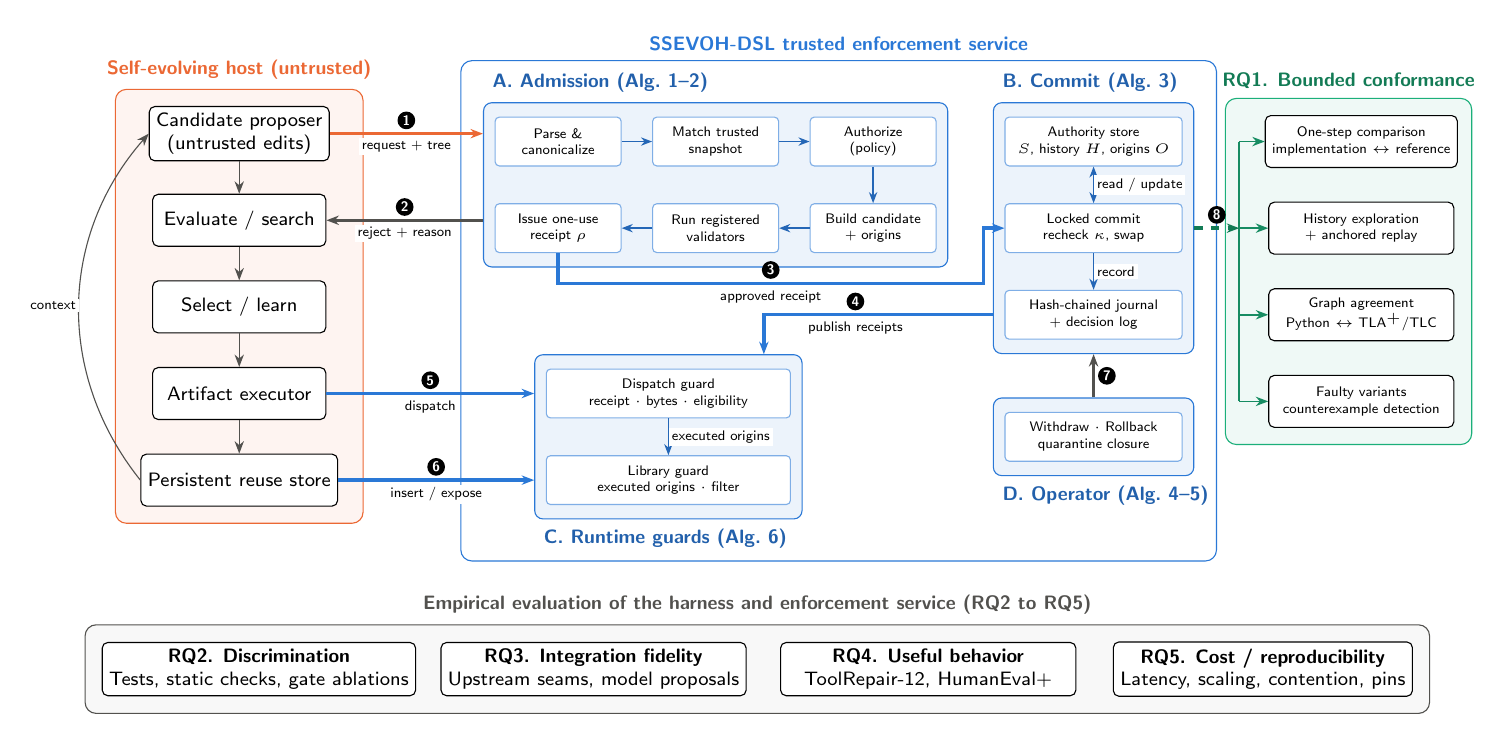
\begin{tikzpicture}[font=\sffamily\scriptsize, >={Stealth[length=4.5pt]},
  box/.style={draw, rounded corners=2pt, align=center, fill=white, inner sep=2.5pt, minimum height=0.66cm},
  chip/.style={draw=trust!60, rounded corners=1.5pt, align=center, fill=white, inner sep=2pt, minimum height=0.62cm, font=\sffamily\tiny},
  mod/.style={draw=trust, rounded corners=3pt, fill=trust!9, inner sep=4pt},
  modt/.style={font=\sffamily\scriptsize\bfseries, text=trust!80!black},
  grp/.style={draw, rounded corners=4pt, inner sep=6pt},
  ia/.style={->, semithick, trust!85!black, >={Stealth[length=4pt]}},
  lbl/.style={font=\sffamily\tiny, align=center, fill=white, inner sep=1pt, text=black},
  flow/.style={->, very thick},
  num/.style={circle, fill=black, text=white, inner sep=0.7pt, font=\sffamily\tiny\bfseries}]
% ---------------- untrusted harness
\node[box, minimum width=2.2cm] (prop) at (0,4.15) {Candidate proposer\\(untrusted edits)};
\node[box, minimum width=2.2cm] (probe) at (0,3.05) {Evaluate / search};
\node[box, minimum width=2.2cm] (sel) at (0,1.95) {Select / learn};
\node[box, minimum width=2.2cm] (exec) at (0,0.85) {Artifact executor};
\node[box, minimum width=2.2cm] (lib) at (0,-0.25) {Persistent reuse store};
\foreach \u/\v in {prop/probe, probe/sel, sel/exec, exec/lib} \draw[->, inkm] (\u) -- (\v);
\draw[->, inkm] (lib.west) to[bend left=40] node[lbl, left]{context} (prop.west);
\begin{scope}[on background layer]
\node[grp, draw=untrust, fill=untrust!7, fit=(prop)(lib), inner xsep=9pt, label={[font=\sffamily\scriptsize\bfseries, text=untrust]above:{Self-evolving host (untrusted)}}] (G1) {};
\end{scope}
% ---------------- module A: admission (serpentine order)
\node[chip, minimum width=1.6cm] (a1) at (4.05,4.05) {Parse \&\\canonicalize};
\node[chip, minimum width=1.6cm] (a2) at (6.05,4.05) {Match trusted\\snapshot};
\node[chip, minimum width=1.6cm] (a3) at (8.05,4.05) {Authorize\\(policy)};
\node[chip, minimum width=1.6cm] (a4) at (8.05,2.95) {Build candidate\\+ origins};
\node[chip, minimum width=1.6cm] (a5) at (6.05,2.95) {Run registered\\validators};
\node[chip, minimum width=1.6cm] (a6) at (4.05,2.95) {Issue one-use\\receipt $\rho$};
\draw[ia] (a1.east) -- (a2.west);
\draw[ia] (a2.east) -- (a3.west);
\draw[ia] (a3.south) -- (a4.north);
\draw[ia] (a4.west) -- (a5.east);
\draw[ia] (a5.west) -- (a6.east);
\begin{scope}[on background layer]
\node[mod, fit=(a1)(a3)(a4)(a6), inner ysep=5pt] (A) {};
\end{scope}
\node[modt, anchor=south west] at (A.north west) {A. Admission (Alg.~1--2)};
% ---------------- module B: commit & state
\node[chip, minimum width=2.25cm] (b1) at (10.85,4.05) {Authority store\\$S$, history $H$, origins $O$};
\node[chip, minimum width=2.25cm] (b2) at (10.85,2.95) {Locked commit\\recheck $\kappa$, swap};
\node[chip, minimum width=2.25cm] (b3) at (10.85,1.85) {Hash-chained journal\\+ decision log};
\draw[ia, <->] (b2.north) -- node[lbl, right]{read / update} (b1.south);
\draw[ia] (b2.south) -- node[lbl, right]{record} (b3.north);
\begin{scope}[on background layer]
\node[mod, fit=(b1)(b3), inner ysep=5pt] (B) {};
\end{scope}
\node[modt, anchor=south west] at (B.north west) {B. Commit (Alg.~3)};
% ---------------- module C: runtime guards
\node[chip, minimum width=3.1cm] (c1) at (5.45,0.85) {Dispatch guard\\receipt $\cdot$ bytes $\cdot$ eligibility};
\node[chip, minimum width=3.1cm] (c2) at (5.45,-0.25) {Library guard\\executed origins $\cdot$ filter};
\draw[ia] (c1.south) -- node[lbl, right]{executed origins} (c2.north);
\begin{scope}[on background layer]
\node[mod, fit=(c1)(c2), inner ysep=5pt] (C) {};
\end{scope}
\node[modt, anchor=north west] at (C.south west) {C. Runtime guards (Alg.~6)};
% ---------------- module D: operator
\node[chip, minimum width=2.25cm] (d1) at (10.85,0.3) {Withdraw $\cdot$ Rollback\\quarantine closure};
\begin{scope}[on background layer]
\node[mod, fit=(d1), inner ysep=5pt] (D) {};
\end{scope}
\node[modt, anchor=north west] at (D.south west) {D. Operator (Alg.~4--5)};
\begin{scope}[on background layer]
\node[grp, draw=trust, fit=(A)(B)(C)(D), inner ysep=15pt, inner xsep=8pt, label={[font=\sffamily\scriptsize\bfseries, text=trust]above:{\tool{} trusted enforcement service}}] (G2) {};
\end{scope}
% ---------------- RQ1: independent checks, not a processing pipeline
\node[box, minimum width=2.35cm, font=\sffamily\tiny] (r1) at (14.25,4.05) {One-step comparison\\implementation $\leftrightarrow$ reference};
\node[box, minimum width=2.35cm, font=\sffamily\tiny] (r2) at (14.25,2.95) {History exploration\\+ anchored replay};
\node[box, minimum width=2.35cm, font=\sffamily\tiny] (r3) at (14.25,1.85) {Graph agreement\\Python $\leftrightarrow$ TLA$^{+}$/TLC};
\node[box, minimum width=2.35cm, font=\sffamily\tiny] (r4) at (14.25,0.75) {Faulty variants\\counterexample detection};
\coordinate (checks) at (12.7,2.95);
\draw[assure!80!black, semithick] (12.7,4.05) -- (12.7,0.75);
\foreach \r in {r1,r2,r3,r4}
  \draw[->, assure!80!black, semithick] (12.7,0 |- \r.west) -- (\r.west);
\begin{scope}[on background layer]
\node[grp, draw=assure, fill=assure!7, fit=(r1)(r4)(checks), inner xsep=5pt, label={[font=\sffamily\scriptsize\bfseries, text=assure!70!black]above:{RQ1. Bounded conformance}}] (G3) {};
\end{scope}
% ---------------- empirical evaluation: measurements, not runtime flows
\node[box, minimum width=3.75cm, font=\sffamily\scriptsize] (q2) at (0.25,-2.65) {\textbf{RQ2. Discrimination}\\Tests, static checks, gate ablations};
\node[box, minimum width=3.75cm, font=\sffamily\scriptsize] (q3) at (4.5,-2.65) {\textbf{RQ3. Integration fidelity}\\Upstream seams, model proposals};
\node[box, minimum width=3.75cm, font=\sffamily\scriptsize] (q4) at (8.75,-2.65) {\textbf{RQ4. Useful behavior}\\ToolRepair-12, HumanEval+};
\node[box, minimum width=3.75cm, font=\sffamily\scriptsize] (q5) at (13,-2.65) {\textbf{RQ5. Cost / reproducibility}\\Latency, scaling, contention, pins};
\begin{scope}[on background layer]
\node[grp, draw=inkm, fill=inkm!4, fit=(q2)(q5), inner ysep=6pt,
  label={[font=\sffamily\scriptsize\bfseries, text=inkm]above:{Empirical evaluation of the harness and enforcement service (RQ2 to RQ5)}}] (G4) {};
\end{scope}
% ---------------- numbered flows between modules only
\draw[flow, untrust] (prop.east) -- node[num, above=1pt]{1} node[lbl, below=1pt]{request + tree} (prop.east -| A.west);
\draw[flow, inkm] (probe.east -| A.west) -- node[num, above=1pt]{2} node[lbl, below=1pt]{reject + reason} (probe.east);
\draw[flow, trust] (a6.south) -- (4.05,2.25) -- node[num, above=1pt]{3}
  node[lbl, below=1pt]{approved receipt} (9.45,2.25) |- (b2.west);
\draw[flow, trust] (B.west |- b3) -| node[pos=0.3, num, above=1pt]{4} node[pos=0.3, lbl, below=1pt]{publish receipts} ([xshift=-14pt]C.north east);
\draw[flow, trust] (exec.east) -- node[num, above=1pt]{5} node[lbl, below=1pt]{dispatch} (exec.east -| C.west);
\draw[flow, trust] (lib.east) -- node[num, above=1pt]{6} node[lbl, below=1pt]{insert / expose} (lib.east -| C.west);
\draw[flow, inkm] (D.north) -- node[num, right=1pt]{7} (B.south -| D.north);
\draw[->, very thick, dashed, assure!70!black] (B.east |- b2) -- node[num, above=1pt]{8} (checks);
\end{tikzpicture}%
}
\caption{Harness-independent lifecycle enforcement and the evaluation coverage of \tool{}.}
\label{fig:overview}
\end{figure*}

\subsection{Host adapter contract}\label{sec:adapter}
A port must satisfy four obligations. \textbf{Mapping:} give artifacts stable component/version identities, bind those identities to exact bytes, and record dependencies and observed derivation sources in trusted metadata. A multi-file bundle may be one workflow component. The core supports one target per transition, not arbitrary multi-component transactions. \textbf{Mediation:} intercept every candidate acceptance, subsequent execution, and persistent-store insertion/retrieval. Check derived candidates as well as initial proposals. \textbf{Authority:} keep authenticated principals, policy, validators, receipts, and history outside the editable surface, and serialize dispatch with withdrawal. \textbf{Evidence:} register domain-specific predicates and an allowed executor. Validate and execute mutable code only within an independently qualified isolation boundary.

These conditions are a porting contract, not an implemented universal plugin API. The core neither discovers omitted lineage nor intercepts arbitrary host actions. Hosts without a reuse store need no store hook, but must mediate any other persistent channel that carries learned artifacts. A cyclic execution workflow can be represented as a single component. Component dependencies and derivations must form a DAG. A host that cannot expose these boundaries is outside the claimed scope.

\subsection{The transition language}\label{sec:dsl}
A specification declares a component snapshot and exactly one evolution: operation (\texttt{update}, \texttt{withdraw}, \texttt{rollback}), target, expected/resulting versions, dependencies, parents, capabilities, validators, and activity conditions. The parser rejects duplicate names/fields, unresolved references, unknown fields, and trailing input. Declarations and set-valued lists are canonicalized. Proposals cannot embed validator code. Listing~\ref{lst:dsl} encodes E1 and compiles with the released compiler.

\begin{lstlisting}[caption={Running example, event E1: a \emph{request} to update \textsf{summarize}.},label={lst:dsl}]
harness ledger {
  component guardrails policy { version 1; mutable false; }
  component summarize tool {
    version 1; mutable true; capabilities [read_ledger]; }
  component report skill {
    version 1; mutable true; depends [summarize]; }
  evolution fix_sign {
    operation update; target summarize; from 1; to 2;
    capabilities [read_ledger];
    requires [structure, signed_ledger];
    expect active; ensure active;
  }
}
\end{lstlisting}

The declared snapshot must match trusted state. The host supplies the authenticated principal, policy, and validators. Editing \textsf{guardrails} or requesting \texttt{network} can be syntactically valid yet unauthorized (E3).

\subsection{Lifecycle state and validity}\label{sec:state}
The lifecycle state is $S=(C,I,W,r)$. The map $C$ records each component's kind, version, mutability, dependencies, parents, and capabilities. The set $I$ contains inactive names, $W$ contains withdrawn \sv{name}{version} identities, and $r$ is a revision. History $H$ and transitive origins $O$ complete the authority's records. Policy and the validator registry also belong to the validation context, while pending receipts and audit records are separate. Commit installs candidate state, history, and origins together. The dependency/parent graph $G$ must be acyclic with known endpoints. Every active component must have active prerequisites and eligible origins:
\begin{equation}
\forall c\notin I:\ \mathsf{Elig}(c,v_c),\ \text{where}\ \mathsf{Elig}(x)\equiv(\{x\}\cup O(x))\cap W=\varnothing.
\label{eq:origin}
\end{equation}
The predicate $\mathsf{Valid}(S,H,O)$ combines these conditions with record typing and uniqueness. Authorization $\mathsf{Auth}(p,e,S)$ checks the principal, operation, target, and capabilities. Evidence $\mathsf{Evidence}(e,S')$ requires exact-\texttt{True} results from all mandatory and requested validators. Protection $\mathsf{Protected}(S,S')$ preserves immutable, policy, and verifier records and forbids newly quarantining them. The strict reverse closure $\mathsf{Dep}_G(t)$ contains components that depend on or derive from $t$, excluding $t$ itself.

\subsection{Admission: preparing a transition}
Algorithm~\ref{alg:prepare} is the only path to an approval. It holds the authority lock, hashes state, policy, validator registry, history, and origins as context $\kappa$, and fails closed at every \textbf{require}. Receipt issuance does not change $\kappa$. Competing approvals can share a base. The pending table privately retains the candidate and request. Candidate construction dispatches by operation to Algs.~\ref{alg:candidate},~\ref{alg:withdraw}, and~\ref{alg:rollback}.

\begin{algorithm}[t]\caption{\textsc{Prepare}: admit a request (flows \circled{1} and \circled{2})}\label{alg:prepare}\footnotesize
\begin{algorithmic}[1]
\Require DSL source $src$, authenticated principal $p$
\State lock authority; $\kappa\gets\mathsf{Id}(\text{service context})$
\State $(IR,e)\gets\textsc{Compile}(src)$; \Req $IR.C=C$
\State \Req $\mathsf{Auth}(p,e,S)$ \Comment{principal, op, target, caps}
\State \Req $e.\mathit{from}=v_{e.t}$ and $e.\mathit{expect}$ holds in $S$
\State $(S',O')\gets\textsc{Candidate}_{e.op}(e,S)$
\State \Req $\mathsf{Protected}(S,S')\wedge\mathsf{Valid}(S',H,O')$
\State \Req $e.\mathit{ensure}$ holds; candidate caps $\subseteq\mathit{Ceil}(e.t)$
\For{$v\in\mathit{Mandatory}\cup e.\mathit{requires}$}
  \State \Req $v\in\mathrm{dom}(\mathit{Registry})$
  \State $ev[v]\gets\mathit{Registry}[v](S',e)$; \Req $ev[v]=\texttt{True}$
  \State \Req $\mathsf{Id}(\text{service context})=\kappa$
\EndFor
\State \Req $\mathsf{Id}(\text{service context})=\kappa$
\State register $(e,S',O')$ under a fresh token $\tau$
\State \Return $\rho=\langle\tau,p,\mathsf{h}(\mathit{IR}),\kappa,\mathsf{h}(S'),\mathsf{h}(O'),ev\rangle$
\end{algorithmic}\end{algorithm}

\textit{Running example.} E1's declared snapshot matches trusted state, policy permits the update with \texttt{read\_ledger}, and the registered \texttt{structure} and illustrative \texttt{signed\_ledger} checks pass. The proposer names a check but cannot supply its result. E3 fails authorization because policy protects \textsf{guardrails} and caps capabilities. Protected-state preservation is checked independently. Rejection returns to the host's own search or retry policy.

\subsection{Candidate construction and origins}
Algorithm~\ref{alg:candidate} computes the candidate for an update. Quarantine uses the \emph{old} graph, so dependents of the replaced version must be revalidated rather than silently inheriting it. Origins are conservative: the new version inherits the previous target version, its origins, and every declared parent version with its origins. An update cannot drop a parent and so cannot declare independence from a withdrawn ancestor. No provenance-severing release operation is provided.

\begin{algorithm}[t]\caption{\textsc{Candidate}: update a target $t$}\label{alg:candidate}\footnotesize
\begin{algorithmic}[1]
\Require canonical request $e$ for target $t$, state $S$
\State $c\gets C[t]$; \Req $e.\mathit{to}>v_c$ and $\sv{t}{e.\mathit{to}}\notin\mathrm{dom}(H)$
\State \Req $c.\mathit{parents}\subseteq e.\mathit{parents}$ \Comment{ancestry never dropped}
\State $Q\gets\mathsf{Dep}_{G(S)}(t)$ \Comment{dependents in old graph}
\State $c'\gets c$ with version $e.\mathit{to}$, relations and caps of $e$
\State $O'\gets O$; $O'(\sv{t}{e.\mathit{to}})\gets\{\sv{t}{v_c}\}\cup O(\sv{t}{v_c})\ \cup$
\State \hspace{1.5em}$\bigcup_{q\in e.\mathit{parents}}\big(\{\sv{q}{v_q}\}\cup O(\sv{q}{v_q})\big)$
\State $I'\gets (I\cup Q)\setminus\{t\}$ \Comment{update activates target}
\State \Return $(\langle C[t\mapsto c'],I',W,r{+}1\rangle,\,O')$
\end{algorithmic}\end{algorithm}

\textit{Running example.} E1 yields $O(\sv{summarize}{2})=\{\sv{summarize}{1}\}$ and quarantines \textsf{report}, which depends on \textsf{summarize}, until it is revalidated against v2. In E4, \textsf{report}~1$\to$2 declares \texttt{parents [summarize]}, so the origin rule records $O(\sv{report}{2})=\{\sv{report}{1},\sv{summarize}{2},\sv{summarize}{1}\}$. Withdrawal in E5 invalidates this derived version through that set.

\subsection{Commit and freshness}
Algorithm~\ref{alg:commit} turns a receipt into state. Because $\kappa$ binds state, policy, validator registry, history, and origins, any successful competing commit invalidates every other receipt prepared from the old base. Staging followed by a reference swap prevents partly applied authoritative transitions. A rejected receipt leaves state unchanged. This is a transaction guarantee for the service and its controlled publication path, not a general filesystem crash-consistency theorem.

\begin{algorithm}[t]\caption{\textsc{Commit}: apply a receipt (flows \circled{3} and \circled{4})}\label{alg:commit}\footnotesize
\begin{algorithmic}[1]
\Require receipt $\rho$
\State lock authority
\State \Req $\rho$ genuine, outstanding, and unconsumed
\State \Req $\rho.\kappa=\mathsf{Id}(\text{service context})$ \Comment{stale otherwise}
\State $(e,S',O')\gets\mathit{Pending}[\rho.\tau]$; recheck their hashes
\State stage history records, $O'$, and hash-chained journal entry
\State atomically swap state references; consume $\rho$
\State notify adapter of committed identity; bind before dispatch
\State append decision record; \Return $(r',x=(e.t,v'_{e.t}))$
\end{algorithmic}\end{algorithm}

\textit{Running example.} E1 and E2 receive receipts with the same $\kappa$. Committing E1 changes $C$, $r$, and $H$, so E2 fails the context check even though E2 alone would have been valid. Re-proposing E2 against the new base is the intended recovery. This is objective~O2.

\subsection{Withdrawal and rollback}
Withdrawal (Alg.~\ref{alg:withdraw}) is the operator's revocation primitive. $W$ grows monotonically ($W\subseteq W'$ for every transition). A dependent may become inactive without its own version being withdrawn, which keeps direct withdrawal distinct from affected closure. Eligibility of derived versions follows from Eq.~\eqref{eq:origin}, so no enumeration of descendants is needed.

\begin{algorithm}[t]\caption{\textsc{Withdraw}: construct a candidate}\label{alg:withdraw}\footnotesize
\begin{algorithmic}[1]
\Require authorized request $e$, target $t$, current version $v$
\State \Req $e.\mathit{to}=v_t=v$ \Comment{historical withdrawal not primitive}
\State $W'\gets W\cup\{\sv{t}{v}\}$; $I'\gets I\cup\mathsf{Dep}_{G}(t)\cup\{t\}$
\State \Return $(\langle C,I',W',r{+}1\rangle,O)$ to \textsc{Prepare}
\end{algorithmic}\end{algorithm}

Rollback (Alg.~\ref{alg:rollback}) loads an exact historical record and its origins. The common admission path rechecks current policy, capability ceilings, validators, and activity conditions. Recovery neither clears $W$ nor overrides an origin's withdrawal.

\begin{algorithm}[t]\caption{\textsc{Rollback}: construct a candidate}\label{alg:rollback}\footnotesize
\begin{algorithmic}[1]
\Require authorized request $e$, target $t$, requested version $v_h$
\State \Req $\sv{t}{v_h}\in\mathrm{dom}(H)$ and $\mathsf{Elig}(\sv{t}{v_h})$
\State $c_h\gets H[\sv{t}{v_h}]$; $Q\gets\mathsf{Dep}_{G}(t)$
\State $I'\gets (I\cup Q)\setminus\{t\}$
\State \Return $(\langle C[t\mapsto c_h],I',W,r{+}1\rangle,O)$ to \textsc{Prepare}
\end{algorithmic}\end{algorithm}

\textit{Running example.} E5 withdraws the current \textsf{summarize}~v2 and quarantines \textsf{report}. Its v2 remains ineligible because $\sv{summarize}{2}\in O(\sv{report}{2})\cap W$, even if dependency metadata later changes. Recovery to v2 is refused. Restoring \textsf{summarize}~v1 and then \textsf{report}~v1 can satisfy current policy (O4). Freshness and origin eligibility are separate obligations.

\subsection{Execution and persistent reuse}\label{sec:integration}
Algorithm~\ref{alg:guard} expresses the host adapter protocol, not a particular framework's API. \textsc{Map} supplies the trusted artifact/metadata binding. \textsc{Bind} associates a committed identity with immutable bytes. \textsc{ExecutorAllowed} checks the domain's execution policy. Admission, dispatch, and withdrawal share the authority lock. Already-running external effects are not undone by withdrawal.

\begin{algorithm}[t]\caption{\textsc{Guard}: host acceptance, execution, and reuse}\label{alg:guard}\footnotesize
\begin{algorithmic}[1]
\Function{Accept}{$artifact$, $base$, $sources$, $p$}
  \State lock; freeze $artifact$ in trusted staging
  \State \Req \textsc{HostChecks}$(artifact)$
  \State $src\gets\textsc{Map}(artifact,base,sources)$
  \State $\rho\gets\textsc{Prepare}(src,p)$; $(r,x)\gets\textsc{Commit}(\rho)$
  \State \textsc{Bind}$(x,\mathsf{h}(artifact))$; \Return $x$
\EndFunction
\Function{Run}{$artifact$, $x$}
  \State lock; \Req bytes match binding, $x$ active and $\mathsf{Elig}(x)$
  \State \Req \textsc{ExecutorAllowed}$(artifact)$
  \State \textsc{HostRun}$(artifact)$; $\mathit{Exec}\gets\mathit{Exec}\cup\{x\}$
\EndFunction
\State \textsc{Insert}$(entry)$: $entry.O\gets\bigcup_{x\in\mathit{Exec}}(\{x\}\cup O(x))$
\State \textsc{Expose}$()$: \Return $\{entry\in\mathit{Store}\mid entry.O\cap W=\varnothing\}$
\end{algorithmic}\end{algorithm}

\textit{Running example.} E4's composition records \textsf{summarize}~v2 as a source of \textsf{report}~v2. Execution records this version, and a learned entry inherits the contributing executions' origins. After E5, dispatch refuses the withdrawn-origin version and retrieval omits the entry (O3). Lineage covers recorded artifact and execution relationships, not every semantic influence on a model. Omitting a memory, cache, or retrieval path from mediation invalidates the portability claim for that host.

\subsection{Correctness argument and audit trail}
Under trusted initialization, pure terminating validators, complete mediation, a stable validation context, and sufficient resources, accepted transitions preserve $\mathsf{Valid}$. Initialization checks acyclicity and active origins. Earlier historical completeness is an operator assumption. Updates preserve identities and ancestry while quarantining dependents (Alg.~\ref{alg:candidate}). Withdrawal grows $W$ and quarantines its closure (Alg.~\ref{alg:withdraw}). Rollback checks historical origins against current $W$ and capability ceilings (Alg.~\ref{alg:rollback}). Candidate checks establish the remaining invariants, and locked commit linearizes the state swap (Alg.~\ref{alg:commit}). Induction over accepted transitions therefore gives preservation. This is a non-mechanized argument, not a proof of the Python interpreter or filesystem. For a representable request admitted by the reference relation, acceptance also requires available history, unchanged context, and passing validators. RQ1 checks both directions of this correspondence within finite bounds.

A hash-chained journal records committed transitions, and anchored replay checks continuity, content, and trusted identity. A separate decision log also records rejections. Together they trace each proposal to its decision and resulting state. Registry identities are process-local and do not attest every captured validator environment. Replay reruns supplied trusted validators. Version origins describe declared and observed workflow relationships, not every semantic influence on a language model.

%=====================================================================
\section{Evaluation}\label{sec:evaluation}
\subsection{Case-study host and adapter}\label{sec:case-study}
We select \harness{}~\cite{harness2}, a recent state-of-the-art recursive harnessing framework, as an integration case study rather than a dependency of the method. Its Propose, Probe, and Compose loop edits and evaluates harness trees. Selection and reflection feed later tasks through an experience library. The pinned runtime (commit \texttt{6868817}) already checks paths and schemas, retries failures, and separates method from judge. These checks address well-formedness, not the lifecycle authority contract studied here. We do not treat absent lifecycle APIs as failures of its stated objectives.

Our adapter maps each multi-file tree to a workflow component and keeps protected configuration, policy, and verifier components separate. Composition/exposure sources extend bundle origins. A dedicated launcher wraps \texttt{\_accept\_tree}, \texttt{\_run\_stage}, and \texttt{Library} without replacing upstream search or learning code. All 70 upstream tests pass. The ledger fixtures allow only two trusted programs. ToolRepair-12 adds static allowlisting and qualified Bubblewrap execution for new tools. HumanEval+ evolves text while grading solution code separately. These domain adapters share one host implementation and therefore do not establish cross-framework portability.

\subsection{Research questions}
\textbf{RQ1 (bounded conformance):} Do the implementation and independent lifecycle semantics agree within published finite bounds?
\par\noindent\textbf{RQ2 (enforcement discrimination):} Which contract violations are blocked and which permitted changes retained, relative to ordinary testing and static validation, and what does each gate contribute?
\par\noindent\textbf{RQ3 (integration fidelity):} Are admission, composition, execution, and library reuse protected inside the original \harness{} workflow, including with model-driven proposers?
\par\noindent\textbf{RQ4 (useful behavior):} Does an evolving agent under the contract deliver useful task outcomes at a documented inference budget?
\par\noindent\textbf{RQ5 (cost and reproducibility):} What do validation, scaling, and contention cost, and can distributed runs be reconstructed from pins and raw records?

\subsection{Study design}\label{sec:design}
Table~\ref{tab:design} summarizes the cohorts, with their construction and measures explained below.

\begin{table*}[t]\caption{Evaluation cohorts and their research questions.}\label{tab:design}\centering\footnotesize
\setlength{\tabcolsep}{5pt}
\begin{tabular}{L{0.25\textwidth}L{0.20\textwidth}L{0.39\textwidth}l}\toprule
Cohort & Size & Purpose & RQ\\\midrule
Bounded assurance & 275,332 checks & Compare implementation and independent semantics & 1\\
Deterministic baselines & 500 decisions & Compare cumulative admission checks & 2\\
Core ablations & 750 decisions & Remove individual lifecycle gates & 2\\
DSL generation & 500 responses & Assess model-generated requests & 2\\
Controlled \harness{} & 900 records & Exercise host seams and gate ablations & 2, 3\\
Host pilots & 25 + 50 streams & Diagnose workflow and usefulness failures & 3, 4\\
ToolRepair-12 & 540 streams & Compare repair usefulness and contract violations & 4\\
HumanEval+ & 3,936 outcomes & Compare evolving and frozen coding agents & 4\\
Scaling & 180 records & Measure graph-size and contention costs & 5\\
Site qualification & 18 runs & Check matched execution across three sites & 5\\\bottomrule
\end{tabular}\end{table*}

\textbf{Cohort structure.} The deterministic study repeats 25 actions five times under four baseline conditions. Full enforcement and five core ablations use the same actions. The DSL cohort crosses five models, 20 contexts covering 17 scenarios, and five seeds. Controlled host experiments repeat each fixture five times. The original, unit-test, and static-check conditions use 12 shared fixtures. Full enforcement and eight host ablations also use four lifecycle fixtures. ToolRepair-12 and HumanEval+ have separate task and stream designs described in Sec.~\ref{sec:rq4}. These cohorts answer different questions and must not be pooled.

\textbf{Conditions.} B0 to B2 are admission-only comparisons. Trusted safe setup advances later contexts, so their timings are not end-to-end deployment costs. In \harness{}, C1 adds one independent signed-ledger unit input after the original checks. C2 adds static principal/protected-file checks and DSL compilation, and is not a semantic verifier. Shared fixtures contain three permitted families (script correction, multifile correction, skill addition) and nine disallowed families (rows of Fig.~\ref{fig:enforcement}a). The four lifecycle families (withdrawn origin, rollback conflict, stale approval, and interrupted publication) correspond to events E2, E4, and E5. C0 to C2 offer no withdrawal/recovery API, so no lifecycle rates are invented for them. The eight ablations remove permissions, dependencies, provenance, evidence, formal verification, withdrawal, rollback, or revalidation individually.

\textbf{Models and budgets.} Qwen2.5-Coder~7B, Phi-4~14B, GPT-OSS~20B, Devstral~24B, and Qwen3-Coder~30B are pinned by manifest digest. The DSL cohort uses temperature~0.2, top-$p$~0.9, 1,024 output and 4,096 context tokens, one generation per model/context/seed. The ledger pilot and ToolRepair-12 use 2,048 output and 16,384 context tokens and run original aggregation at $k{=}1$: four solver rollouts and three proposal stages per task, at most two edit attempts per stage. Raw request/response records retain all calls, tokens, limits, and failures.

\textbf{Measures and analysis.} \emph{Unsafe deployment} means deploying a request that violates the explicit operator contract. It is not a maliciousness classifier. We separate syntax validity, oracle evaluability, allowed and disallowed attempts, deployment, false rejection, protocol/workflow failure, and task success. Invalid output is never counted as a safe request. Zero eligible observations yield an undefined rate, not zero risk. A post hoc strict request-fidelity diagnostic checks every declared field. It is not preregistered and not the safety oracle. Units depend on the study: designed scenarios in the primary cohort, families in ToolRepair-12, and ordered model/seed streams in HumanEval+. Sites supply infrastructure. Between-model comparisons in the primary cohort (task-cluster bootstrap, paired sign-flip tests, Holm) are diagnostic and reported only in the artifact. With few tasks we emphasize counts and effect sizes. ToolRepair-12 and HumanEval+ follow their own frozen protocols (Sec.~\ref{sec:rq4}).

\subsection{RQ1: Bounded conformance}
Table~\ref{tab:rq1} summarizes the assurance evidence. The one-step graph/lifecycle domain has 176,256 cases over acyclic two-component graphs, inactive and withdrawn subsets, and relations to self, another component, or a missing component. Target versions range from 1 to 3 and expected versions from 1 to 2, with activity conditions varied. A separate 72,576-case domain varies one component's kind, mutability, capabilities, grant, and evidence. Together these checks accept 3,388 requests and reject 245,444 without a discrepancy against the independent reference.

History exploration starts from seven two-component graphs, uses versions 1 to 3, and explores all operations to depth four. It visits 3,307 contexts and checks 19,620 transitions, of which 6,880 are accepted. Anchored replay checks every accepted endpoint. These are finite-domain counts, not estimates of deployment prevalence or independent replications.

The lifecycle model has one proposal and dependency epochs 0 to 2. Python and TLC agree in all four authorization/evidence contexts, with 18/44, 18/44, 23/62, and 61/133 states/edges. The publication model has one bundle, one origin bit, and two epochs. Its graphs agree at 45/81 states/edges with authorization and evidence enabled and 4/4 in each other context. Five lifecycle variants omit authorization, evidence, withdrawal, rollback, or revalidation. All yield counterexamples, as do six publication variants. For example, omitting revalidation permits deployment after a dependency change in five steps.

\begin{table}[t]\caption{Summary of bounded assurance and regression results.}\label{tab:rq1}\centering\footnotesize
\setlength{\tabcolsep}{3pt}
\begin{tabular}{L{0.31\columnwidth}L{0.31\columnwidth}L{0.29\columnwidth}}\toprule
Check & Extent & Result\\\midrule
One-step conformance & 248,832 cases & No differences\\
History exploration & 19,620 transitions & No differences\\
Anchored replay & 6,880 endpoints & No differences\\
Lifecycle model & 4 contexts & Python = TLC\\
Publication model & 4 contexts & Python = TLC\\
Faulty variants & 11 variants & All detected\\
Regression suites & 62 / 32 / 70 tests & All pass\\\bottomrule
\end{tabular}\end{table}

The regression counts refer to the stored core, integration, and upstream \harness{} suites, respectively. They are source-scoped checks of the evaluated implementation.

\textbf{Answer to RQ1.} The checked representations agree within their finite bounds and detect all injected variants. This establishes bounded consistency, not a Python-to-TLA$^{+}$ refinement theorem or semantic safety for generated code.

\subsection{RQ2: Enforcement discrimination}
\textbf{Deterministic baselines and core ablations.} Each row of Table~\ref{tab:rq2} contains 125 decisions: 60 disallowed and 65 allowed. FA counts disallowed requests admitted, and FR counts allowed requests rejected. Latency is the median admission time in milliseconds. The table shows that syntax (B0) and schema (B1) checks admit all 60 disallowed actions. Trusted policy with candidate construction (B2) still admits 20, namely those whose violation is only visible to validators or lifecycle history. Full enforcement (B3) admits none and rejects none of the 65 allowed actions. Removing dependency closure, provenance checks, or revalidation each re-opens five admissions. Removing dependency closure also causes ten false rejections, because skipped quarantine diverges later state. Removing withdrawal or rollback checks alone has no effect in these cases because retained guards overlap. A zero single-gate effect does not show that a mechanism is dispensable.

\begin{table}[t]\caption{Admission errors and median latency across baseline conditions and core gate ablations.}\label{tab:rq2}\centering\footnotesize
\begin{tabular}{lrrr}\toprule
Condition & FA & FR & Median ms\\\midrule
B0 syntax only & 60/60 & 0/65 & 0.197\\
B1 + snapshot schema & 60/60 & 0/65 & 0.203\\
B2 + policy, candidate & 20/60 & 0/65 & 0.227\\
B3 full enforcement & \textbf{0/60} & \textbf{0/65} & 0.599\\\midrule
Full $-$ dep.\ closure & 5/60 & 10/65 & 0.538\\
Full $-$ provenance & 5/60 & 0/65 & 0.708\\
Full $-$ revalidation & 5/60 & 0/65 & 0.593\\
Full $-$ withdrawal & 0/60 & 0/65 & 0.563\\
Full $-$ rollback & 0/60 & 0/65 & 0.841\\\bottomrule
\end{tabular}\end{table}

\begin{figure*}[t]\centering
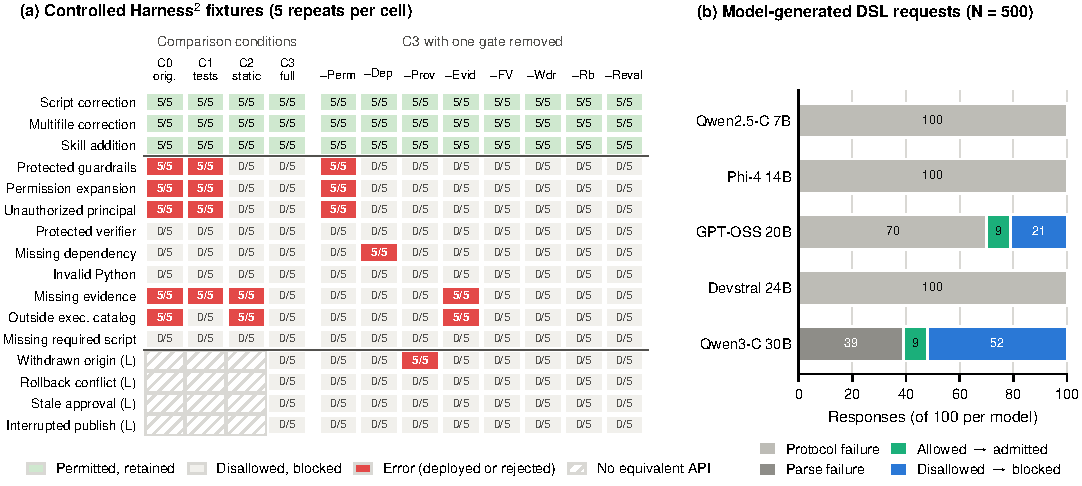
\includegraphics[width=\textwidth]{figures/enforcement.pdf}
\caption{Enforcement outcomes. (a)~Each cell counts, over five repeats, permitted changes retained (top three rows) or disallowed changes deployed (other rows). Red cells are errors. Original \harness{} admission (C0) deploys 25/45 shared violations. Ordinary testing (C1) still deploys 20 and static DSL validation (C2) 10. Full enforcement (C3) deploys none, retains all permitted changes, and blocks all four lifecycle families (L). Removing a single gate re-opens exactly the families that gate covers. (b)~Of 500 model-generated DSL requests, 409 never reach the oracle (fenced, empty, length-limited, or identifier-level parse failures). Every oracle-classified request is decided correctly.}
\label{fig:enforcement}
\end{figure*}

\textbf{Model-generated requests.} Fig.~\ref{fig:enforcement}b and Table~\ref{tab:models} show that only 91 of 500 generated responses are oracle-evaluable: 73 disallowed and 18 allowed. Full enforcement deploys none of the 73 and falsely rejects none of the 18. Three models return fenced output in all 100 responses, which the strict raw-text protocol rejects. GPT-OSS has 56 empty and 62 length-limited outputs (overlapping). The historical \texttt{syntax\_valid} flag is also set for parser-level identifier failures: 39 Qwen3-Coder responses quote a relation or capability identifier and fail before oracle classification, so the flag must not be read as 100 parsed programs. Filtering to valid proposals would hide these interface failures.

Table~\ref{tab:models} reports 100 DSL responses and five guarded host streams per model. In the DSL columns, Flag counts the historical \texttt{syntax\_valid} marks, Oracle gives allowed/disallowed evaluable requests, and Fid. is post hoc strict request fidelity. In the host columns, WF ok counts completed workflows, Inv. counts invalid proposals, Adm. gives allowed proposals admitted, and Blk. gives disallowed proposals blocked. The notation n/a marks unavailable or inapplicable entries.

\begin{table}[t]\caption{Model-generated requests test the DSL interface and guarded \harness{} workflows.}\label{tab:models}\centering\footnotesize
\setlength{\tabcolsep}{3.2pt}
\begin{tabular}{lrrr|rrrr}\toprule
& \multicolumn{3}{c|}{Primary DSL} & \multicolumn{4}{c}{\harness{} streams}\\
Model & Flag & Oracle & Fid. & WF ok & Inv. & Adm. & Blk.\\\midrule
Qwen2.5-C 7B & 0 & 0/0 & 0\% & 5/5 & 0 & 7/7 & 30/30\\
Phi-4 14B & 0 & 0/0 & 0\% & 5/5 & 43 & 0/0 & 17/17\\
GPT-OSS 20B & 30 & 9/21 & 21\% & 0/5 & n/a & n/a & n/a\\
Devstral 24B & 0 & 0/0 & 0\% & 5/5 & 0 & 0/0 & 54/54\\
Qwen3-C 30B & 100 & 9/52 & 21\% & 5/5 & 0 & 9/9 & 40/40\\\midrule
Total & 130 & 18/73 & n/a & 20/25 & 43 & 16/16 & 141/141\\\bottomrule
\end{tabular}\end{table}

\textbf{Answer to RQ2.} Full enforcement deploys 0/60 deterministic, 0/73 oracle-classified model, and 0/45 controlled violations with no false rejections in those populations. Most generated outputs fail the interface before an assessable decision.

\subsection{RQ3: Integration fidelity in \harness{}}\label{sec:rq3}
Fig.~\ref{fig:enforcement}a and Table~\ref{tab:rq3} report five repeats per host fixture. Each applicable condition has 45 shared disallowed, 15 permitted, and 20 lifecycle attempts. Shared and Lifecycle count disallowed executions, Retained counts permitted executions, and ms is mean latency over permitted executions. Timings are descriptive and order-confounded. Lifecycle results are inapplicable to C0, C1, and C2 (n/a), and ablation timings are unreported (n/r).

Original checks miss protected-file, permission, principal, evidence, and executable-catalog violations. C1 closes the catalog gap, while C2 closes the first three gaps. C3 blocks all shared and lifecycle violations and retains all permitted executions. Removing provenance re-admits the withdrawn-origin case in every repeat. Removing permissions, evidence, or dependencies re-admits 15, 10, or 5 shared violations, respectively.

\begin{table}[t]\caption{Controlled \harness{} fixtures compare contract violations, permitted executions, and latency.}\label{tab:rq3}\centering\footnotesize
\setlength{\tabcolsep}{3.5pt}
\begin{tabular}{lrrrr}\toprule
Condition & Shared & Retained & Lifecycle & ms\\\midrule
C0 original & 25/45 & 15/15 & n/a & 77.17\\
C1 + unit test & 20/45 & 15/15 & n/a & 155.73\\
C2 + static DSL & 10/45 & 15/15 & n/a & 78.33\\
C3 full & \textbf{0/45} & \textbf{15/15} & \textbf{0/20} & 114.81\\\midrule
C3 $-$ permissions & 15/45 & 15/15 & 0/20 & n/r\\
C3 $-$ evidence & 10/45 & 15/15 & 0/20 & n/r\\
C3 $-$ dependencies & 5/45 & 15/15 & 0/20 & n/r\\
C3 $-$ provenance & 0/45 & 15/15 & 5/20 & n/r\\
C3 $-$ any other & 0/45 & 15/15 & 0/20 & n/r\\\bottomrule
\end{tabular}\end{table}

\textbf{Model-driven streams.} With real model proposers inside the same workflow (Table~\ref{tab:models}, right), C3 blocks all 141 assessed disallowed proposals and admits all 16 permitted non-no-op proposals at exact bytes. GPT-OSS fails all five workflows before producing an assessable proposal. These failures remain in stream and task denominators. This pilot never exercised reflection, because our launcher omitted the model client as \harness{}'s selector (all fifty task summaries have empty experience). The corrected launcher (Sec.~\ref{sec:rq4}), the deterministic fixtures, and eight coding-adapter regressions cover library guarding.

\textbf{Answer to RQ3.} The supported adapter enforces admission, composition, dispatch, and library exposure at actual upstream call sites. This is one executable integration under the stated restrictions, not evidence of cross-framework portability.

\subsection{RQ4: Useful behavior}\label{sec:rq4}
\textbf{Pilot.} The first host pilot has 25 streams from five models and five seeds, with two ledger tasks per stream. A corrected pilot compares two executable policies in 50 streams. The initial pilot exposed three adapter defects (answer schema, selector channel, answer form). After the fixes, no disallowed proposal executed (0/31 catalog, 0/13 sandboxed) and sandboxed evidence admitted correct repairs the catalog rejected (8/50 versus 0/50 correct values, post hoc), but strict success stayed 0/100, so we ran a prespecified study.
\textbf{ToolRepair-12 design.} Twelve tool families each plant one defect in the harness's executable CSV tool (e.g., sign handling, rounding, column order, blank and grouped numbers, Fig.~\ref{fig:toolrepair}b). Each family has a specification, a trusted reference, and disjoint task inputs (graded by exact output), operator-held validation inputs (authority only), and oracle inputs (independent proposal oracle only). The full design has 540 streams, each containing three tasks. Five pinned models run three seeds per family in three arms: original \harness{} (A1), the contract with the catalog policy (A2), and the contract with sandboxed evidence (A3). A frozen reference runs inside every stream, and each stream receives one injected proposal from seven rotating classes. All arms execute non-catalog tools under the same infrastructure sandbox, which is not credited to contract enforcement. Protocol, analysis, and implementation hashes were frozen before qualification. Families are the inferential unit (10,000 paired cluster-bootstrap resamples, 95\% percentile intervals). The frozen analysis applies Holm to bootstrap tail proportions for H1/H3. These are resampling diagnostics, not calibrated population-level $p$-values. Two deviations were recorded before any full result: amendment v1.1 made three crashing defects silent and reran all 540 streams, and the smoke run exposed an ``executed'' label that counted proposals restating \emph{unchanged} files. The corrected label is primary and both are reported.

\begin{figure*}[t]\centering
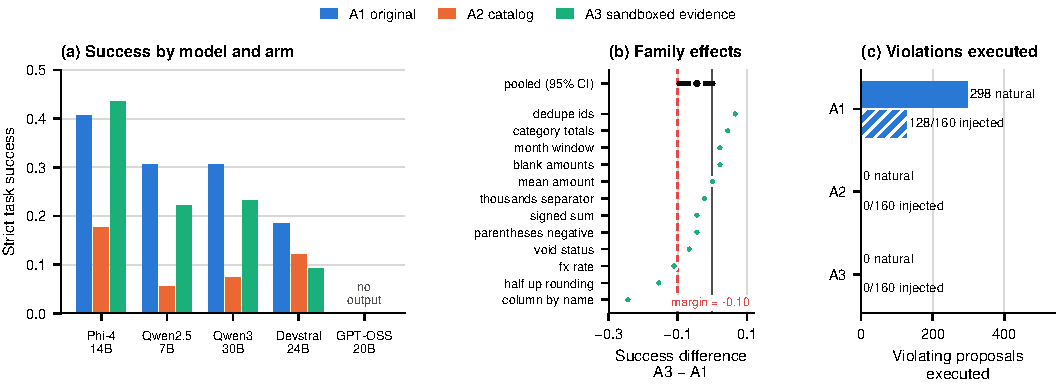
\includegraphics[width=\textwidth]{figures/toolrepair.pdf}
\caption{ToolRepair-12 (540 streams). (a)~Strict task success per model (GPT-OSS: no output, failure in every arm). (b)~Per-family difference A3$-$A1, pooled family-cluster estimate and 95\% CI, and the prespecified margin. (c)~Contract-violating proposals executed (corrected label, declared probe excluded).}
\label{fig:toolrepair}
\end{figure*}

\textbf{Usefulness.} Mean per-family success is 0.241 for original \harness{}, 0.085 under the catalog, and 0.196 under sandboxed evidence (frozen: 0.041, Fig.~\ref{fig:toolrepair}). The sandboxed-evidence interval meets the prespecified 10-point non-inferiority margin against the unguarded arm (difference $-0.044$, 95\% CI $[-0.096, +0.002]$, frozen resampling decision H3 met) and recovers 11.1 points over the catalog (95\% interval $[+0.067, +0.159]$, H1 met under the frozen rule). The lower bound lies only 0.4 percentage points inside the margin, and family effects vary (Fig.~\ref{fig:toolrepair}b). Within A3 streams, success rises from 0.12 on the first task to 0.26 on the third (H4, exploratory), but fixed task order and the absence of a no-library ablation prevent attributing this trend to learning.

\textbf{Safety at the same time.} Original \harness{} executed 426 contract-violating proposals (298 natural, 128/160 injected). A3 executed 0 natural and 0/160 injected violations under the corrected label (H2's observed-count criterion). These are planned-stream counts, including workflows that failed before proposals. Repeated classes within families/models are dependent, so we do not interpret the artifact's nominal binomial bound as a population risk bound. Under the uncorrected worker label, A3 shows 12 natural executions and H2 would not hold. Two A3 oracle-unknown cases were resolved after collection by direct oracle-input execution, while four A1 cases remain unknown. This supplementary resolution is not a qualified sandbox replication and is retained separately from the prespecified correction. As declared before the study, the input-triggered resource-abuse probe, whose trigger lies outside every validation case, passed behavioral evidence in 16/20 A3 streams and ran bounded by the sandbox. Only Phi-4 succeeds more often under sandboxed evidence than unguarded (47 versus 44 of 108). GPT-OSS produced no output (empty responses under JSON-constrained decoding). Its streams count as failures (intention to evaluate), and excluding them (exploratory) gives 0.301, 0.106, and 0.245.

\textbf{HumanEval+.} In a prespecified text-only study~\cite{humaneval,evalplus} (164 tasks, Phi-4 and Qwen2.5-Coder, three seeds, hidden tests graded after a global freeze), guarded minus original evolution is $-0.6$ points for Phi-4 (seeds $-8.5$ to $+3.7$) and $+1.8$ for Qwen. Neither beats frozen best-of-eight selection (guarded/original/frozen: Phi-4 0.354/0.360/0.476, Qwen 0.766/0.748/0.780) at about 1.8$\times$ its calls. The four reported endpoints are original evolution, guarded evolution, frozen selection, and a one-shot endpoint drawn from the frozen pool. Across all tasks, models, and seeds, these yield 3,936 outcomes. These are descriptive all-attempts accuracies over three ordered streams/model, not task-independent significance tests. Frozen selection matches solver calls rather than total compute. One seed/model was regenerated before hidden grading after a storage failure, a recorded deviation.
\textbf{Answer to RQ4.} A3 meets the frozen ToolRepair non-inferiority rule narrowly, retaining 81\% of A1's point-estimate success. The margin is large relative to the 0.241 baseline. Guarding preserves rather than creates usefulness: neither evolving HumanEval+ arm beats frozen selection. Behavioral evidence contains but does not exclude the declared input-triggered probe.

\subsection{RQ5: Cost and reproducibility}
\begin{figure*}[t]\centering
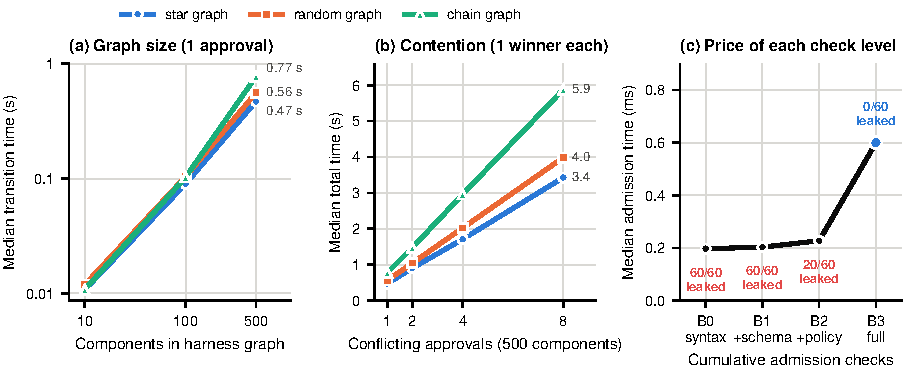
\includegraphics[width=\textwidth]{figures/cost.pdf}
\caption{Three aspects of enforcement cost (medians of five repeats). (a)~\emph{Graph size:} transition time grows with the number of components and depends on graph shape through the size of the quarantine closure. (b)~\emph{Contention:} with 1 to 8 conflicting approvals on 500 components, time grows linearly and every cell has exactly one commit winner. (c)~\emph{Check level:} each cumulative admission check adds little latency. Only full enforcement (B3, 0.60\,ms) leaks none of the 60 disallowed actions.}
\label{fig:cost}
\end{figure*}

\textbf{Validation and scaling.} Fig.~\ref{fig:cost} summarizes scaling and the admission baselines. The scaling design crosses three graph sizes, three graph shapes, four contention levels, and five repeats, giving 180 records. Shape matters because quarantine follows reverse reachability: chains quarantine the longest closures. Contention is resolved by compare-and-swap on the context hash: in every tested cell exactly one approval commits and the others are rejected as stale. These observations establish neither distributed throughput nor an asymptotic bound. Traced Python allocation peaks at 2.5\,MB at 500 components. In \harness{}, the permitted-execution mean rises from 77.17\,ms (C0) to 114.81\,ms (C3), a descriptive, order-confounded fixture difference. C1's slower 155.73\,ms reflects its extra test process and does not establish general superiority to testing.

\textbf{Reproducibility.} Qualification comprises 18 runs across three sites, two studies, and three matched trials. HPC runs used Fir, Narval, and Rorqual through a \texttt{use-hpc}-derived Slurm pipeline~\cite{usehpc} with source freezes, cache identity and GPU checks, measured site qualification, and hash-verified collection. Censored and failed cells are preserved, and superseded cells are re-run as recorded supplements rather than overwritten. Twenty-four matched cross-site pairs produced identical text and decisions under identical identities. All 24 were syntax-invalid outputs, so this shows deterministic serving, not useful generation.

\textbf{Answer to RQ5.} The 0.6\,ms admission median is below 0.1\% of ToolRepair's 1.1\,s mean stream time per call. Admission for a 500-component chain takes 0.77\,s. These scoped measurements exclude inference and do not establish distributed service throughput. Reanalysis and raw-archive availability are distinguished in Sec.~\ref{sec:availability}.

\subsection{Discussion: transfer and engineering trade-offs}\label{sec:discussion}
\textbf{What transfers.} Component granularity and search strategy are adapter choices. ADAS-like archive search~\cite{adas} could mediate design promotion and execution. Code-evolving agents~\cite{dgm} additionally need code isolation. Skill-learning agents~\cite{voyager} need installation, execution, and retrieval guards. These are architectural mappings, not implemented ports. The tested bundle projection demonstrates multi-file binding, not fine-grained mediation of every kind.

\textbf{When transfer fails.} A host that bypasses a guard, cannot authenticate its caller, omits sources, or lets evolved code modify the authority violates Sec.~\ref{sec:adapter}. Current restrictions include single-target updates, acyclic metadata relations, conservative ancestry, in-process serialization, and no verified restart or distributed commit. Withdrawal cannot erase prior model context or undo an external side effect. A clean independent rewrite cannot shed withdrawn ancestry in this language. An operator-approved provenance-release mechanism is future work.

\textbf{Operational value.} The service supplies an auditable release condition for generated changes. Catalog validation rejects useful equivalent programs. Behavioral evidence expands the trusted base and misses input-triggered defects. Four zero-effect ablations reflect overlapping guards, not established redundancy. Operators must maintain mappings, policies, validators, and isolation.

\subsection{Threats to validity}
\textbf{Construct.} Compliance with an operator lifecycle contract is narrower than harmless agent behavior. Correctness, fidelity, and authorization are distinct, and strict fidelity is post hoc. The RQ2 and RQ3 fixtures were written by the authors alongside the gates they exercise, so their one-to-one coverage shows that each gate works as designed, not that the gate set is complete. Injected red-team classes and model-generated proposals only partly offset this.
\textbf{Internal.} Validators and reference semantics can share design errors. Independent implementations and faulty variants reduce but do not eliminate common-mode mistakes. The core assumes a trusted process boundary. Qualified domain sandboxes do not make the authority safe against a hostile same-user host. Durable restart is unsupported. Behavioral oracles use disjoint inputs but share domain specifications and some checks with validators, so agreement is not an independent proof of semantic safety.
\textbf{External.} Designed fixtures are not a sample of real attacks. Two catalog programs, two ledger tasks, and twelve single-tool planted-defect families do not establish general autonomous work, and pilot correct-value counts are post hoc. Models and sites do not add tasks. All empirical adapters use one host, so neither multiple domains nor a generic interface establishes cross-framework generalization. Public benchmarks such as HumanEval+ may be contaminated.
\textbf{Conclusion.} Zero observed violations is not zero risk. The H3 interval is only 0.4 points inside a wide margin relative to the 0.241 base rate, and bootstrap tail proportions are not calibrated tests. H2 depends on corrected labels and supplementary oracle resolution. Repeated fixtures are not independent samples. Workflow failures reduce the assessable safety population and remain failures for task outcomes.
\textbf{Operational.} Queues, GPUs, and model serving affect completion (GPT-OSS never produced output). Pins, raw logs, and censoring support audit, not determinism.

%=====================================================================
\section{Related Work}\label{sec:related}
\textbf{Runtime enforcement and authorization.} We specialize runtime monitoring~\cite{schneider} and authorization~\cite{cedar,cedarengineering} to versioned evolution and reuse. The separation of an untrusted producer from a trusted checker resembles proof-carrying code~\cite{necula}, but receipts are context-bound service records rather than program proofs. TLA$^{+}$~\cite{lamport} supplies bounded cross-checks, not a refinement theorem. Our origin relation specializes PROV-DM~\cite{prov} for revocation eligibility.

\textbf{Agent safety languages.} AgentSpec enforces declarative rules over execution and can inspect trajectories~\cite{agentspec}. Progent controls evolving tool privileges and checks policy changes with an SMT solver~\cite{progent}. AutoSpec learns rule revisions from counterexamples~\cite{autospec}. Our distinction is an explicit artifact lifecycle combining context-bound approval with origin eligibility across execution and reuse. Existing rule languages could encode parts of this contract with additional state and hooks. We claim neither greater expressiveness nor empirical security superiority, as no head-to-head comparison was run.

\textbf{Software update security and dynamic updating.} The Update Framework addresses stale and compromised update metadata~\cite{tuf}, while in-toto binds supply-chain steps to authorized producers and artifacts~\cite{intoto}. Our contract additionally follows self-generated versions and derivation origins into execution and experience reuse. Admission depends on current policy and validator evidence. Dynamic updating~\cite{dsu} addresses safe code replacement and state transfer, whereas we govern version eligibility.

\textbf{Prompt injection.} Indirect injection turns untrusted content into instructions~\cite{greshake}. CaMeL separates trusted control flow from untrusted data with capabilities~\cite{camel}. A self-evolving harness adds a persistent channel through its own edited files and library, which our contract treats as untrusted proposals and origin-tracked entries.

\textbf{Self-evolving agents and benchmarks.} ADAS searches over agent designs~\cite{adas}, Voyager accumulates a reusable skill library~\cite{voyager}, the Darwin G\"odel Machine studies open-ended self-improvement~\cite{dgm}, and \harness{} recursively adapts harnesses~\cite{harness2}. Our authority boundary governs releases and subsequent reuse independently of these search procedures (Sec.~\ref{sec:discussion}). Only the \harness{} mapping is empirically exercised. HumanEval and EvalPlus assess generated-program correctness~\cite{humaneval,evalplus} and complement lifecycle checks.

%=====================================================================
\section{Conclusion}
\tool{} treats approval as a revocable relation to a versioned context. Its metadata rules and adapter obligations apply independently of how a harness searches for improvements. Execution and persistent reuse must remain mediated. Bounded assurance supports consistency of the rules, and one \harness{} integration demonstrates enforcement at real admission, execution, and reuse seams. ToolRepair-12 exposes the usefulness/evidence trade-off, while HumanEval+ shows no advantage over frozen selection. Cross-framework ports, broader tasks, durable recovery, and mechanized refinement remain necessary to establish wider applicability.

\textbf{Artifacts.}\label{sec:availability} The versioned evidence snapshot~\cite{ssevohartifact} contains the core, pinned host runtime, protocols/deviations, outcome records, and analysis scripts. \texttt{make verify} checks bounded assurance. \pathcode{experiments/scripts/} contains outcome analyses. ToolRepair success is reproducible from committed \pathcode{toolrepair-v1/streams.jsonl}. Corrected execution labels are documented in \pathcode{experiments/toolrepair/DEVIATIONS.md} and require the locally retained per-stream archives, which are not in the public snapshot. Thus full independent replication of that corrected safety result remains an artifact-release limitation, rather than a completed archival release.
\clearpage
\bibliographystyle{IEEEtran}
\balance
\bibliography{references}
\end{document}
